\documentclass[10pt,conference,compsocconf]{IEEEtran}

\usepackage{hyperref}
\usepackage{graphicx}	% For figure environment


\begin{document}
\title{Machine Learning - Project 1}

\author{
  Marion Chabrier, Valentin Margraf, Octavianus Sinaga\\
  \textit{Department of Computer Science, EPFL Lausanne, Switzerland}
}

\maketitle

\begin{abstract}
The goal of this project is to apply Machine Learning techniques on data from CERN generated by smashing protons into one another and measuring the decay signature of the possibly resulted Higgs boson. With this decay signature as input our model predicts whether it actually was result of a Higgs boson or something else (noise). We use different regression methods to tackle this problem. We got F-1 score 0.728 and accuracy 0.822 by implementing least square as the best result amongst other methods that we implemented.
\end{abstract}

\section{Introduction}
First we preprocess the data i.e. standardize it and get rid of missing values and outliers.
Then we implement the six different methods: Least Squares, Least Squares GD, Least Squares SGD, Ridge Regression, Logistic Regression, Regularized Logistic Regression. We use each method to learn a model on the training data and see how well they perform. For each model we additionally vary the hyperparameters to optimize the performance. Finally we compare their performances on the test data from CERN by submitting it on AICrowd.



\section{Data Preprocessing}
\label{sec:prepro}
In order to deal with the data, we need to standardize it. The standardization helps us to scale the data in a bounded interval. We standardize both, the test and the train data set. \\
We afterwards delete outliers: values, which are further away from the mean than a certain threshold. 
\\
The preprocessing deals with:
\begin{itemize}
	\item Substitution of the -999 values for each entries using the mean of \textit{clean} data in train and test dataset
	\item Normalizing/standardizing the value for all entries with standar deviation and mean
	\item Deletion of outliers in the train data (set the treshold to cut off the entries)
\end{itemize}

\begin{figure}[htbp]
	\centering
	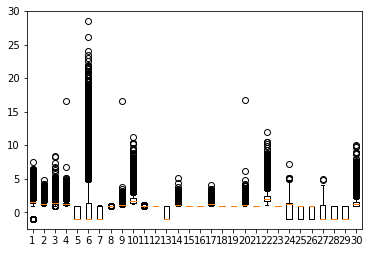
\includegraphics[width=\columnwidth]{trainBoxPlot.png}
	\caption{Boxplot for train dataset. )
	\vspace{-3mm}
	\label{fig:prepro}
\end{figure}



\begin{figure}[htbp]
	\centering
	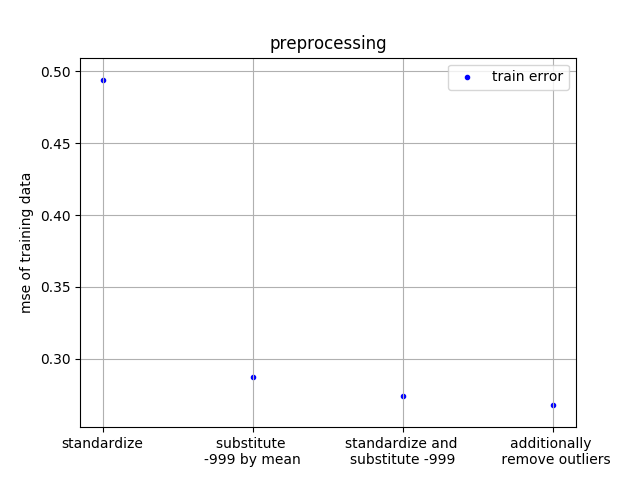
\includegraphics[width=\columnwidth]{preprocessing.png}
	\caption{MSE for different approaches of preprocessing using least squares to evulate their effect.}
	\vspace{-3mm}
	\label{fig:prepro}
\end{figure}


In order to find out, which approaches of preprocessing yield good results, we evaluate their effect on the MSE. In figure 1 we used Least Squares to demonstrate this. In can be observed, that just standardizing does not help us to preprocess the data in a good way because the MSE is still quiet high. 
By substituting the -999 values by the mean of the data, a big reduction in the loss can be achieved. Furthermore the loss can be reduced by standardizing the data and removing outliers. For removing outlier, we plotted the boxplot to observe the quantiles of each features. and we use this value as threshold to filter out the outlier of each data point.\\



\section{Methods}
\label{sec:tips-writing}


For each model we run 4-fold cross validation on our training data to tune our hyperparameters in order to optimize our model. The hyperparameters in this case are the \textit{degree} for all the models and the constant \textit{lambda} for the Ridge Regression and the Regularized Logistic Regression.
\\
Figure 2 shows how the choice of the \textit{degree} affects the \textit{RMSE} in the case of Least Squares. We run the cross validation for degrees between 1 and 13 and find out, that for degree = 11 we get our best result. For higher degrees the model will overfit and lower degrees instead give a bigger \textit{RMSE}, hence the model underfits.

\begin{figure}[htbp]
  \centering
  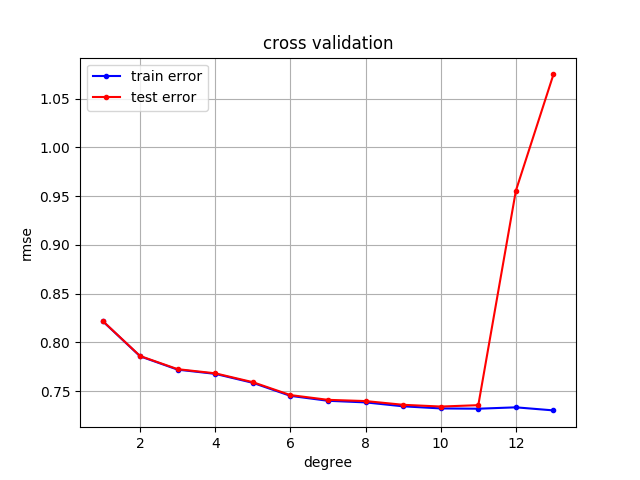
\includegraphics[width=\columnwidth]{cross_validation_leastsquares.png}
  \caption{RMSE for different degrees using Least Squares.}
  \vspace{-3mm}
  \label{fig:crossvalidationleastsquares}
\end{figure}


\begin{figure}[htbp]
	\centering
	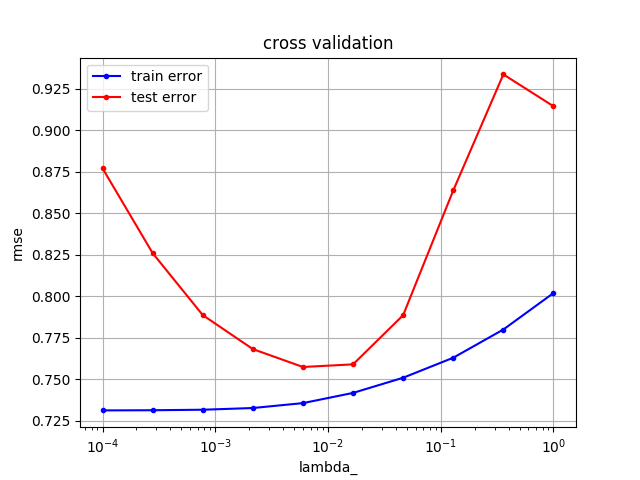
\includegraphics[width=\columnwidth]{cross_validation_ridge_degree_12.png}
	\caption{RMSE for different lambdas using ridge\_regression (degree 12).}
	\vspace{-3mm}
	\label{fig:crossvalidationridge}
\end{figure}
 %%%%pic to be added
 %%% find optimal lambda
 For the Ridge Regression a degree of 12 gives the best result. Using cross validation we computed the \textit{RMSE} for different values of \textit{lambda} in order to optimize this second hyperparameter. We find out, that a value of approximately 0.0059 gives the best result, which can be checked in Figure 3. When we choose this value too small, the test error gets much bigger, whereas the training error reduces. If \textit{lambda} is too big, both, the test and training error augment.\\
 The final used hyperparameter for each method can be found in table 1.\\


\begin{table}[htbp]
	\centering
	\begin{tabular}[c]{|l||l|l|}
		\hline
		Methods&degree&lambda\\
		\hline
		Least Squares& 11 &-\\
		Least Squares GD& 10 & -\\
		Least Squares SGD & 10 &-\\		Ridge Regression&12&0.00599\\
		Logistic Regression & 10&-\\
		Reg. Logistic Regression&10&0.01\\
		\hline
	\end{tabular}
	\caption{Optimized hyperparameters computed\\ through 4-fold cross validation.}
	\label{tab:hyperpam}
\end{table}

\newpage

\section{Results}


After having optimized the hyperparameters for each model we want to see how the different models perform on the test data from CERN. We therefore submit each prediction on \textit{AICrowd} and see what result it gives us. In table 2 they can be compared.


\begin{table}[h]
	\centering
	\begin{tabular}[c]{|l||l|l|}
		\hline
		Methods&Accuracy&F1-Score\\
	\hline
	Least Squares&0.822&0.728\\
	Least Squares GD&0.682&0.511\\
	Least Squares SGD&0.391&0.394\\		
	Ridge Regression&0.815&0.713\\
	Logistic Regression&0.819&0.718\\
	Reg. Logistic Regression&0.819&0.717\\
	\hline
	\end{tabular}
	\caption{Performances of our models submitted on AICrowd.}
	\label{tab:perform}
\end{table}

Ending up with an accuracy of 0.822 and F1-Score of 0.728, Least Squares performs best amongst all methods. Least Squares Gradient and Stochastic Gradient methods in contrast perform not very well. 
Ridgre regression performs quite good as well, it gives an accuracy of 0.815 and F1-Score of 0.713.
Logistic and Regularized Logistic Regression give both an accuracy of approx. 0.67 but perform quite bad when taking the F1-Score as accuracy measure. 


\section{Discussion}

 
Least Squares Gradient performs not as good as the Least Squares method, even though in theory it would converge to the same optimum. We had to choose a quite small \textit{gamma} (approx $10^{-19}$) for not making explode the loss. The stepsize can be concerned as an additional hyperparameter which to choose correctly. The Least Squares Stochastic Gradient Descent performs even worse. Reasons for that might be also badly chosen stepsize \textit{gamma} and batchsize.\\
We did not take computational cost into account and Least Squares gave us a good result. That's why we did not focus that much on optimizing the stepsize in order to make the both Gradient methods perform better. \\
Logistic Regressions and Regularized Logistic Regression perform quite similar which is actually surprising, given the fact that the additional penalty term is supposed to avoid overfitting, hence to support simpler models. But since we ended up with an optimal degree of 10 for both methods, we might have chosen \textit{lambda} to small to have a real impact.


\section{Summary}

In this project we used different regression methods to predict the Higgs Boson. After preprocessing the data and optimizing the hyperparameters for each method using 4-fold cross validation, we have chosen the Least Squares Method to tackle this task. This method performed best concerning Accuracy and F1-Score.



%\bibliographystyle{IEEEtran}
%\bibliography{literature}

\end{document}
